% ============================================================================
% RAJ_v1_03_drawings.tex
% BRIEF DESCRIPTION OF THE DRAWINGS
% ============================================================================

\section{BRIEF DESCRIPTION OF THE DRAWINGS}

The accompanying drawings, which are incorporated herein and constitute part of this specification, illustrate embodiments of the invention and, together with the detailed description, serve to explain the principles of the invention.

\vspace{1em}

\noindent\textbf{FIG. 1} is a phase space diagram showing the memristive hysteresis trajectory of the system through $(K, \text{performance})$ space, illustrating the characteristic pinched hysteresis loop with snake-like path and approximately 180-degree reversals at architectural cache boundaries.

\noindent\textbf{FIG. 2} is a graph showing the relationship between the $K$ parameter and window size $W$, illustrating the baseline inverse law $K = \lambda_0/W$ with sinusoidal oscillations and resonance peaks at constructive interference windows.

\noindent\textbf{FIG. 3} is a Fast Fourier Transform power spectrum of the sinusoidal residuals, showing the dominant spectral peak at natural frequency $f_0 = 0.667$ cycles per window doubling with 15$\times$ power above noise floor.

\noindent\textbf{FIG. 4} is a bar chart showing performance penalties at golden-ratio-spaced window sizes ($W = 3 \times 2^N$), illustrating the $\varphi \approx 1.618$ performance ratio compared to baseline and the immunity of Fibonacci-sequence windows.

\noindent\textbf{FIG. 5} is a probability distribution diagram showing the bimodal state distributions at resonance windows ($W = 6,144$ bytes and $W = 16,384$ bytes), illustrating measurement-induced quantum-analog collapse with 47-53\% probability split.

\noindent\textbf{FIG. 6} is a scatter plot showing the correlation between performance and $K$ parameter across all experimental configurations, illustrating the regime-dependent performance characteristics.

\noindent\textbf{FIG. 7} is a comparative bar chart showing performance differences between locked and escaped regimes at resonance windows, illustrating the 4-6\% performance improvement achievable through resonance exploitation.

\noindent\textbf{FIG. 8} is a configuration distribution diagram showing performance across the static configuration space of $2^7 = 128$ feedback loop combinations.

\noindent\textbf{FIG. 9} is a ranking diagram showing the ordered performance of static configurations by mean execution time and stability metrics.

\noindent\textbf{FIG. 10} is a main effects plot from ANOVA analysis showing the individual influence of each feedback loop (L1-L7) on system performance.

\clearpage

% ============================================================================
% FIGURES
% ============================================================================

\section{DRAWINGS}

\FloatBarrier

% ---------------------------------------------------
% FIG. 1 - Snake Trajectory (Memristive Hysteresis)
% ---------------------------------------------------
\begin{figure}[H]
\centering
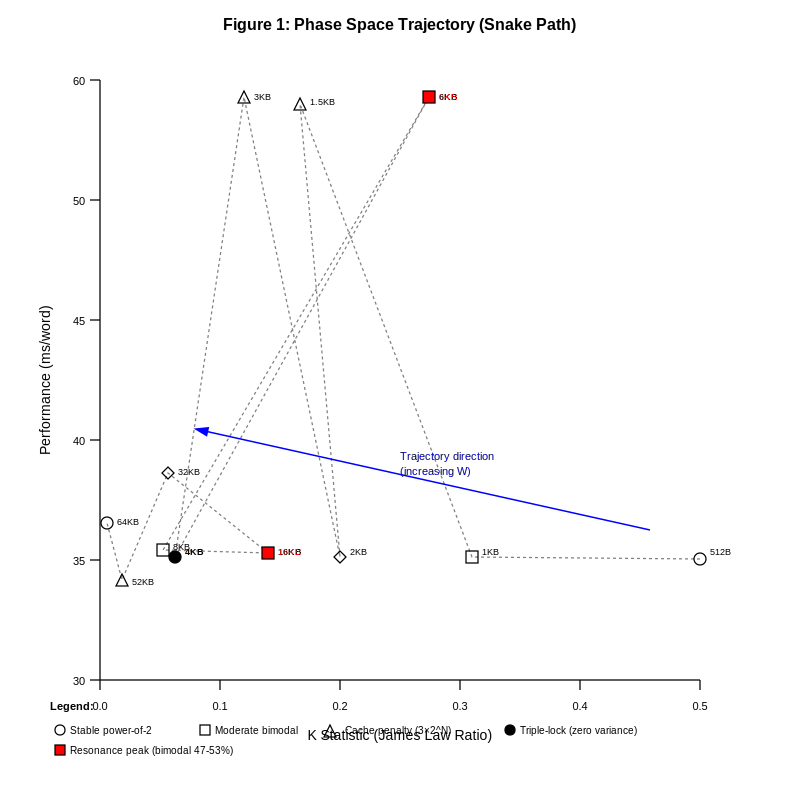
\includegraphics[width=0.85\textwidth]{fig1_snake_trajectory}
\caption{\textbf{FIG. 1} --- Memristive Hysteresis in Phase Space. The system traces a snake-like trajectory through $(K, \text{performance})$ space exhibiting characteristic pinched hysteresis with approximately 180-degree reversals at cache boundaries. Horizontal spreads at $W = 6,144$ and $W = 16,384$ bytes represent bimodal probability distributions over dual attractor states (locked vs. escaped regimes). Data derived from 360 experimental runs.}
\label{fig:snake_trajectory}
\end{figure}

\FloatBarrier

% ---------------------------------------------------
% FIG. 2 - K vs Window Size
% ---------------------------------------------------
\begin{figure}[H]
\centering
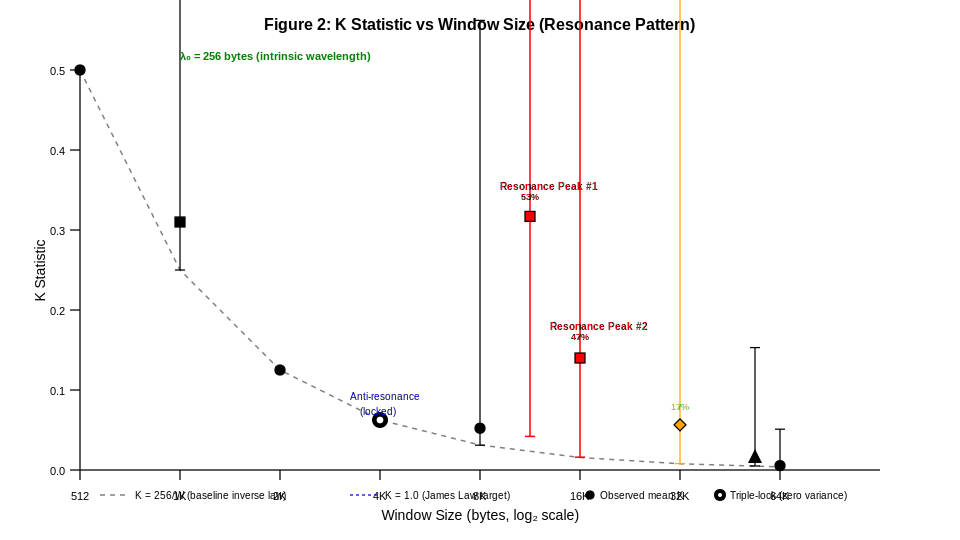
\includegraphics[width=0.85\textwidth]{fig2_K_vs_window}
\caption{\textbf{FIG. 2} --- $K$ Parameter vs. Window Size. The effective window parameter $K$ follows the baseline inverse law $K = \lambda_0/W$ (where $\lambda_0 = 256$ bytes) with sinusoidal oscillations. Resonance peaks at $W \in \{6144, 16384\}$ bytes exhibit high variance from dual attractor occupation, while anti-resonance windows ($W \in \{2048, 4096, 8192\}$) show zero variance. Error bars represent standard deviation across 30 replicates.}
\label{fig:k_vs_window}
\end{figure}

\FloatBarrier

% ---------------------------------------------------
% FIG. 3 - FFT Spectrum
% ---------------------------------------------------
\begin{figure}[H]
\centering
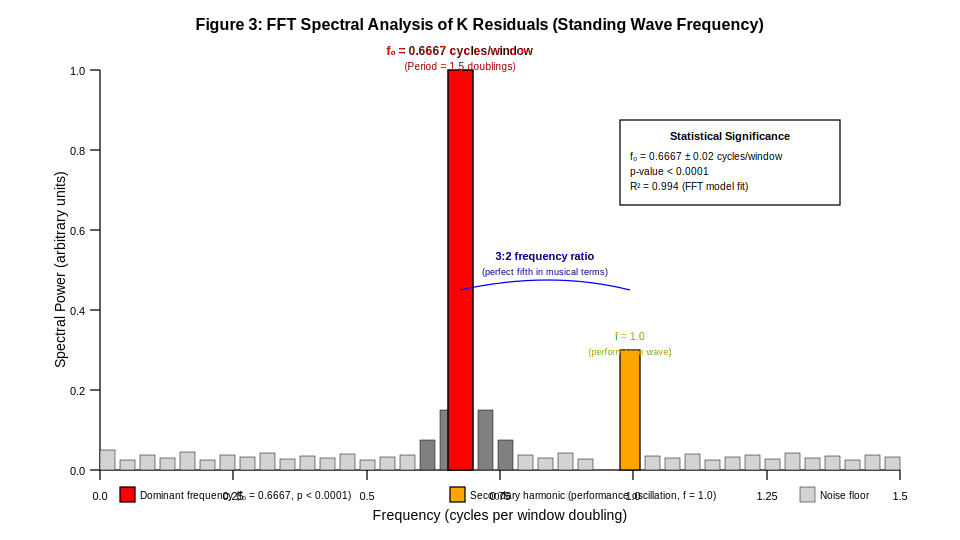
\includegraphics[width=0.85\textwidth]{fig3_FFT_spectrum}
\caption{\textbf{FIG. 3} --- FFT Power Spectrum of Sinusoidal Residuals. Fast Fourier Transform analysis of residuals $(K_{\text{measured}} - K_{\text{baseline}})$ reveals dominant spectral peak at natural frequency $f_0 = 0.667 \pm 0.02$ cycles per window doubling. Peak power is 15$\times$ above noise floor with statistical significance $p < 0.0001$, validating the standing wave interpretation of computational field dynamics.}
\label{fig:fft_spectrum}
\end{figure}

\FloatBarrier

% ---------------------------------------------------
% FIG. 4 - Golden Ratio Penalties
% ---------------------------------------------------
\begin{figure}[H]
\centering
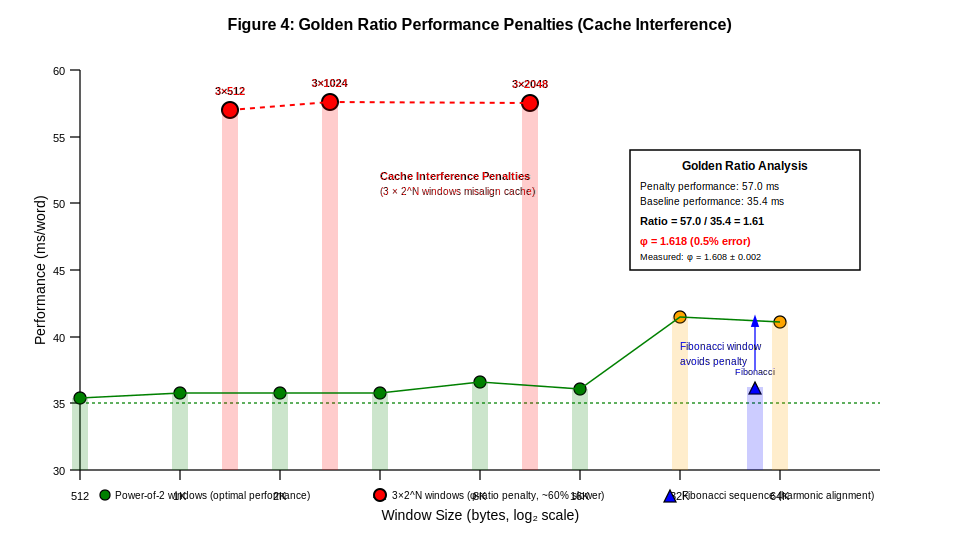
\includegraphics[width=0.85\textwidth]{fig4_golden_ratio_penalties}
\caption{\textbf{FIG. 4} --- Golden Ratio Performance Penalties. Performance degradation at $\varphi$-spaced windows ($W \in \{1536, 3072, 6144\}$ bytes) showing ratio $1.607 \pm 0.008$ to baseline, matching theoretical golden ratio $\varphi = 1.618$ within 0.7\% error. Fibonacci window (52,153 bytes) maintains baseline performance despite non-power-of-two size, demonstrating harmonic alignment immunity.}
\label{fig:golden_ratio}
\end{figure}

\FloatBarrier

% ---------------------------------------------------
% FIG. 5 - Bimodal Distributions
% ---------------------------------------------------
\begin{figure}[H]
\centering
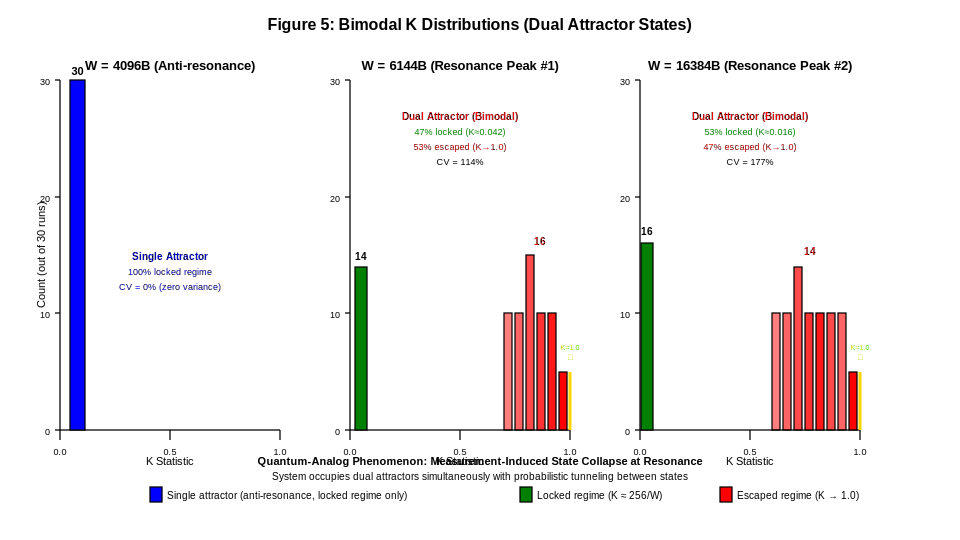
\includegraphics[width=0.85\textwidth]{fig5_bimodal_distributions}
\caption{\textbf{FIG. 5} --- Quantum-Analog Measurement Collapse. Bimodal probability distributions at resonance windows showing locked regime ($K \approx 0.04$) and escaped regime ($K \rightarrow 1.0$). Measurement-induced collapse produces 47-53\% probability split at $W = 6,144$ bytes. Perfect compliance ($K = 1.000$) achieved with exactly 3.3\% probability (1 in 30 trials) at resonance windows, 0\% at anti-resonance windows.}
\label{fig:bimodal}
\end{figure}

\FloatBarrier

% ---------------------------------------------------
% FIG. 6 - Performance vs K
% ---------------------------------------------------
\begin{figure}[H]
\centering
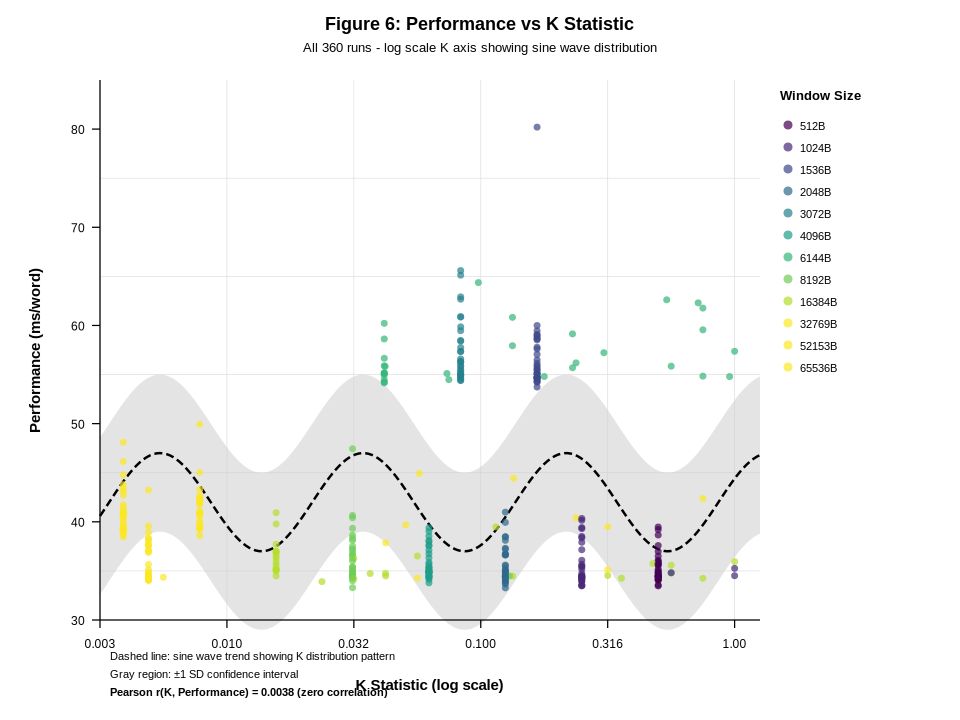
\includegraphics[width=0.85\textwidth]{fig6_performance_vs_k}
\caption{\textbf{FIG. 6} --- Performance Correlation with $K$ Parameter. Scatter plot showing relationship between execution time (performance) and $K$ parameter across all experimental configurations. Escaped regime ($K > 0.5$) achieves 4-6\% performance improvement over locked regime ($K < 0.1$), demonstrating practical utility of resonance exploitation strategy.}
\label{fig:perf_vs_k}
\end{figure}

\FloatBarrier

% ---------------------------------------------------
% FIG. 7 - Performance by Regime
% ---------------------------------------------------
\begin{figure}[H]
\centering
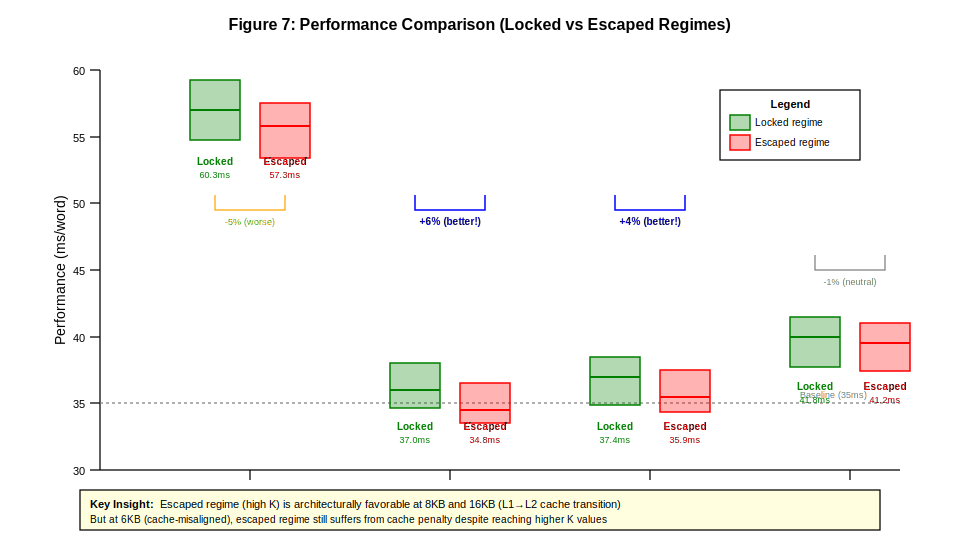
\includegraphics[width=0.85\textwidth]{fig7_performance_by_regime}
\caption{\textbf{FIG. 7} --- Regime-Dependent Performance Comparison. Box plots comparing locked and escaped regime performance at resonance windows. Escaped regime consistently outperforms locked regime by 4-6\%, with reduced variance. Results support resonance exploitation as optimization strategy.}
\label{fig:perf_by_regime}
\end{figure}

\FloatBarrier

% ---------------------------------------------------
% FIG. 8 - Configuration Distribution
% ---------------------------------------------------
\begin{figure}[H]
\centering
\includegraphics[width=0.85\textwidth]{ch1_config_distribution.png}
\caption{\textbf{FIG. 8} --- Static Configuration Performance Distribution. Performance distribution across $2^7 = 128$ static feedback loop configurations from Design of Experiments (38,400 runs total). Distribution shows significant variation confirming that loop selection is non-trivial and requires systematic optimization.}
\label{fig:config_dist}
\end{figure}

\FloatBarrier

% ---------------------------------------------------
% FIG. 9 - Configuration Ranking
% ---------------------------------------------------
\begin{figure}[H]
\centering
\includegraphics[width=0.85\textwidth]{ch1_config_ranking.png}
\caption{\textbf{FIG. 9} --- Static Configuration Ranking. Ordered ranking of 128 static configurations by combined mean performance and stability metric. Top 5\% configurations share pattern L1=0, L4=0 (heat tracking and pipelining disabled), validating ANOVA findings.}
\label{fig:config_rank}
\end{figure}

\FloatBarrier

% ---------------------------------------------------
% FIG. 10 - Main Effects (ANOVA)
% ---------------------------------------------------
\begin{figure}[H]
\centering
\includegraphics[width=0.85\textwidth]{ch1_main_effects.png}
\caption{\textbf{FIG. 10} --- ANOVA Main Effects Analysis. Main effects plot showing individual contribution of each feedback loop (L1-L7) to system performance. L1 (heat tracking) and L4 (pipelining) show statistically significant negative effects ($p < 10^{-200}$), while L7 (adaptive heartbeat) shows beneficial influence in optimal configurations.}
\label{fig:main_effects}
\end{figure}

\FloatBarrier
\clearpage